\documentclass[a4paper,class=article,border=5pt,tikz]{standalone}
\usetikzlibrary{calc}

\tikzset{% define a style to shift coordinates
  s/.style={every coordinate/.try}
}

%sqrt(2)/2 = 0.7071067812

\begin{document}
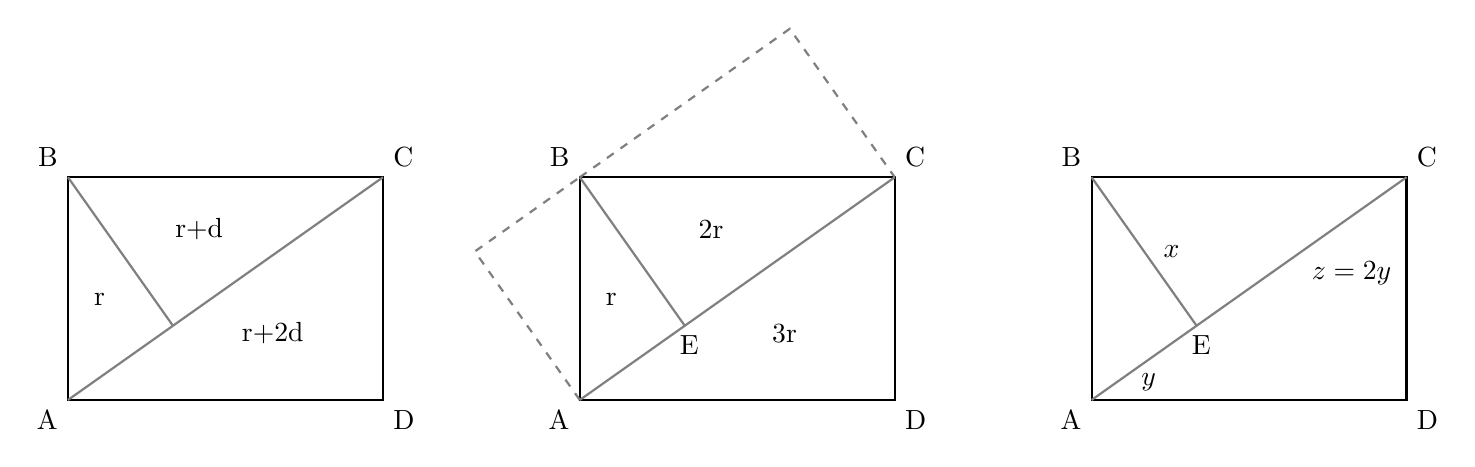
\begin{tikzpicture}[thick, scale=1]
% coordinates to be reused
\coordinate (A) at (0,0);
\coordinate (B) at (0,0.7071*4);
\coordinate (C) at (4,0.7071*4);
\coordinate (D) at (4,0);
\path (B) -- ($(A)!(B)!(C)$) coordinate (E); 
\path let \p1 = (E) in coordinate (F) at (-\x1,0.7071*4cm-\y1);
\path let \p1 = (E) in coordinate (G) at (4cm-\x1,2*0.7071*4cm-\y1);

% draw first picture
\node [below left] at (A) {A};
\node [above left] at (B) {B};
\node [above right] at (C) {C};
\node [below right] at (D) {D};
\draw (A) -- (B) -- (C) -- (D) -- cycle;
\draw [gray] (A) -- (C);
\draw [gray] (B) -- (E); 
\node at ($(A)!0.5!(D)!0.3!(C)$) {r+2d};
\node at ($(B)!0.5!(E)!0.3!(C)$) {r+d};
\node at ($(A)!0.5!(B)!0.3!(E)$) {r};

% draw second picture
\begin{scope}[every coordinate/.style={shift={(6.5,0)}}]
\node [below left] at ([s]A) {A};
\node [above left] at ([s]B) {B};
\node [above right] at ([s]C) {C};
\node [below right] at ([s]D) {D};
\draw ([s]A) -- ([s]B) -- ([s]C) -- ([s]D) -- cycle;
\draw [gray] ([s]A) -- ([s]C);
\draw [gray] ([s]B) -- ([s]E);
\node at ($([s]A)!0.5!([s]D)!0.3!([s]C)$) {3r};
\node at ($([s]B)!0.5!([s]E)!0.3!([s]C)$) {2r};
\node at ($([s]A)!0.5!([s]B)!0.3!([s]E)$) {r};
\node [below] at ([s]E) {~E};
\draw [gray,dashed] ([s]A) -- ([s]F) -- ([s]B);
\draw [gray,dashed] ([s]B) -- ([s]G) -- ([s]C);
\end{scope}


% draw third picture
\begin{scope}[every coordinate/.style={shift={(13,0)}}]
\node [below left] at ([s]A) {A};
\node [above left] at ([s]B) {B};
\node [above right] at ([s]C) {C};
\node [below right] at ([s]D) {D};
\draw ([s]A) -- ([s]B) -- ([s]C) -- ([s]D) -- cycle;
\draw [gray] ([s]A) -- ([s]C);
\draw [gray] ([s]B) -- ([s]E);
\node [below] at ([s]E) {~E};
\node [right] at ($([s]B)!0.5!([s]E)$) {~$x$};
\node [below] at ($([s]A)!0.5!([s]E)$) {~$y$};
\node [below right] at ($([s]C)!0.5!([s]E)$) {$z=2y$};
\end{scope}

\end{tikzpicture}
\end{document}
